\documentclass[10 pt,usenames,dvipsnames, oneside]{article}
\usepackage{../../../modelo-ensino-medio}



\begin{document}

\begin{center}
  \begin{minipage}[l]{3cm}

\includegraphics[width=2cm]{logo}    
\end{minipage}\hfill
\begin{minipage}[r]{.8\textwidth}
 {\Large \scshape Atividade: Colhendo Estrelas}  
\end{minipage}
\end{center}
\vspace{.2cm}

\ifdefined\prof
%Habilidades da BNCC
% \begin{objetivos}
% \item 
% \end{objetivos}

%Caixa do Para o Professor
\begin{goals}
%Objetivos específicos
\begin{enumerate}
\item Reconhecer as transformações geométricas associadas a
parâmetros aplicados às expressões analíticas das funções
seno e no esboço do seu gráfico.
\item Explorar o gráfico da função seno por meio de uma
ferramenta digital
\end{enumerate}

\tcblower

%Orientações e sugestões
\begin{itemize}
\item Professor, ao longo do livro viemos utilizando o GeoGebra e
agora usaremos outra ferramenta gráfica. Não tem problema,
nesse contexto, elas são muito similares.
\end{itemize}
\end{goals}

\bigskip
\begin{center}
{\large \scshape Atividade}
\end{center}
\fi

Usando o link da plataforma Desmos (\url{https://teacher.desmos.com/activitybuilder/custom/566b317d4e38e1e21a10ab07\#preview/df77bcd1-a128-4e8b-a1e6-6417acf42950}), altere os parâmetros da função seno para alterar o formato da senóide e conseguir pegar todas as estrelas da tela.

\begin{figure}[H]
\centering

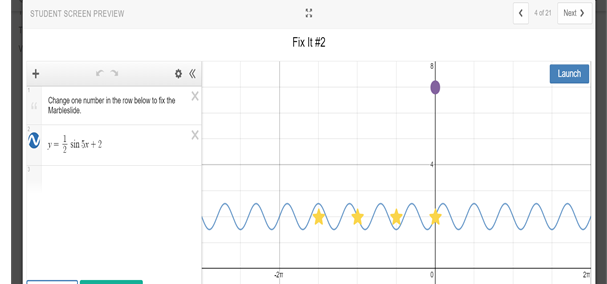
\includegraphics[width=.8\linewidth]{trigonometricas97}
\caption{Fonte: \href{https://teacher.desmos.com/activitybuilder/custom/566b317d4e38e1e21a10ab07\#preview/df77bcd1-a128-4e8b-a1e6-6417acf42950}{Desmos -- Marbleslides: Periodics}}
\label{}
\end{figure}

\ifdefined\prof
\begin{solucao}

O gabarito dela consta no próprio site.

\end{solucao}
\fi

\end{document}